% ============================
% CONFIGURACIÓN DEL DOCUMENTO
% ============================
\documentclass[spanish,authorshippage=ltd]{thesis} % Clase de documento específica para tesis


% ============================
% PAQUETES UTILIZADOS
% ============================
\usepackage{masterthesis}    % Plantilla específica para tesis
\usepackage{titlesec}        % Personalización de títulos y secciones
\usepackage{pgfplots}        % Gráficos en coordenadas matemáticas
\usepackage{graphicx}        % Inclusión de imágenes
\usepackage{appendix}        % Manejo de anexos
\usepackage{rotating}        % Rotación de elementos
\usepackage{tabularray}      % Tablas avanzadas
\usepackage{lipsum}          % Texto de relleno
\usepackage{tablefootnote}   % Notas al pie en tablas
% Paquetes matemáticos
\usepackage{amssymb}
\usepackage{latexsym}
\usepackage{amsmath}
\usepackage{csquotes}


% Paquetes para algoritmos
\usepackage{algorithm}
\usepackage{algorithmic}

% Paquetes para imágenes y gráficos
\usepackage{epsfig}          % Manejo de imágenes EPS
\usepackage{epstopdf}        % Conversión de EPS a PDF
\usepackage{graphics}        % Soporte adicional para gráficos
\usepackage{ps4pdf}          % Soporte para PostScript
\usepackage{float}           % Control de posición de imágenes
\usepackage{pgf}             % Creación de gráficos vectoriales
\usepackage{afterpage}       % Control de paginación

% Configuración de código fuente con listings
\usepackage{listings,newtxtt} % Resaltado de código
\lstset{
	extendedchars=true,
	language=Python,
	basicstyle=\footnotesize\ttfamily,
	showstringspaces=false,
	showspaces=false,
	numbers=left,
	numberstyle=\footnotesize,
	numbersep=9pt,
	tabsize=2,
	breaklines=true,
	showtabs=false,
	captionpos=b,
	basicstyle=\ttfamily, 
	keywordstyle=\bfseries,
	morekeywords={self,import,print},
	xleftmargin=15pt,
	xrightmargin=0pt,
	emph={MyClass,__init__}
}

% ============================
% DEFINICIÓN DE COMANDOS
% ============================
\newcommand\blankpage{%
	\null
	\thispagestyle{empty}%
	\addtocounter{page}{-1}%
	\newpage}

% Configuración de gráficos con PGFPLOTS
\pgfplotsset{
	textnumber/.style={
		/pgf/number format/.cd,
		fixed,
		fixed zerofill,
		precision=4,
		1000 sep={ },
	},
}

% Definición de operadores matemáticos personalizados
\newtheorem{definition}{Definición}
\DeclareMathOperator*{\argmax}{arg\,max}
\DeclareMathOperator*{\argmin}{arg\,min}

% Formato de subpárrafos
\titleformat{\subparagraph}
{\normalfont\normalsize\bfseries}{\thesubparagraph}{1em}{}
\titlespacing*{\subparagraph}{\parindent}{3.25ex plus 1ex minus .2ex}{.75ex plus .1ex}

% ============================
% INFORMACIÓN DEL DOCUMENTO
% ============================
\addauthor{Daniel Rojas Grass}
\title{{\normalsize Multiagente Conversacional para la interacción con los datos del transporte marítimo recogidos en el Diario de la Marina.}}
\ucicenter{Centro de Informatización Gobierno-Empresa}
\facultynum{1}
\addtutor[Tutor]{Dr.C. Orlando Grabiel Toledano López}
\addtutor[Tutores]{MsC. Olga Yarisbel Rojas Grass}
\addtutor[Tutores]{Ing. Keren Saray Naranjo}

% ============================
% SECCIONES INICIALES
% ============================
\acknowledgment{
	Agradecimientos y cita inspiradora:
	\begin{flushright}
		\textbf{\textit{"La ciencia es mi vida (...) moriría por ella". Nikolái Ivánovich Vavílov}}
	\end{flushright}
}

\abstract{Resumen de la tesis.}
\keywords{Palabras clave}

% ============================
% ESTRUCTURA DEL DOCUMENTO
% ============================
\begin{document}
	
	% ========================
	% PORTADA Y SECCIONES PRELIMINARES
	% ========================
	\begin{titlepage}
		\begin{figure}
			\centering
			
\includegraphics[width=0.25\linewidth]{images/uci}
		\end{figure}
		\centering{\textsc{\large UNIVERSIDAD DE LAS CIENCIAS INFORMÁTICAS}     \\
			\textsc{\large CENTRO DE INFORMATIZACIÓN GOBIERNO-EMPRESA} \\
			\textsc{\large FACULTAD DE TECNOLOGIAS LIBRES} \\}
		\vspace{3cm}
		\centering\textsc{\large Multiagente Conversacional para la interacción con los datos del transporte marítimo recogidos en el Diario de la Marina.\\}
		\vspace{2cm}
		\centering{\bfseries Tesis presentada en opción al grado científico de \\
			Ingeniero en Ciencias Informáticas\\}
		\vspace{2.5cm}
		\centering{\bfseries Autor:\\}
		\centering{Daniel Rojas Grass\\}
		\vspace{0.5cm}
		\centering{\bfseries Tutores:\\}
		\centering{
			Dr.C. Orlando Grabiel Toledano López\\
			MsC. Olga Yarisbel Rojas Grass\\
			Ing. Keren Saray Naranjo\\
		}	
		\vspace{2cm}
		\centering{ \bfseries La Habana, febrero del 2025}
		
	\end{titlepage}
	
	\pagenumbering{roman}
	\authorshipdeclared

\parskip 10pt 
\spacing{1.5} 
\setlength{\parindent}{0pc}

El autor del trabajo de diploma con título  \textit{\textbf{“Multiagente conversacional para la interacción con los datos del transporte marítimo recogidos en el Diario de la Marina”}}, concede a la Universidad de las Ciencias Informáticas los derechos patrimoniales de la investigación, con carácter exclusivo. De forma similar se declara como único autor de su contenido.

Y para que así conste, firmo la presente declaración jurada de autoría en La Habana a los \rule{8mm}{0.2mm} días del mes de \rule{30mm}{0.2mm} del año \rule{15mm}{0.2mm}.


\vspace{1in}

\begin{center}
	\rule{60mm}{0.3mm} \\
	\textbf{Daniel Rojas Grass}
\end{center}

%\bigskip
\vspace{0.5in}

\begin{center}
	\begin{tabular}{cp{0.5in}c}		
		\rule{65mm}{0.3mm}      &   & \rule{65mm}{0.3mm}        \\
		%\cargoTutor &   & \cargoCoTutor \\
		\textbf{Dr.C. Orlando Grabiel Toledano López}      &   & \textbf{MsC. Olga Yarisbel Rojas Grass}
	\end{tabular}
\end{center}

%\bigskip
\vspace{0.5in}

	\contactdata

\parskip 10pt \spacing{1.5} \setlength{\parindent}{0pc}

Curriculum e información de contacto del tutor: nombre y apellidos, títulos académicos, formación de postgrado recibida, lugar de trabajo, responsabilidades laborales asumidas, experiencia profesional, líneas de trabajo y/o investigación, correo electrónico, perfiles en redes profesionales

Curriculum e información de contacto del asesor: nombre y apellidos, títulos académicos, formación de postgrado recibida, lugar de trabajo, responsabilidades laborales asumidas, experiencia profesional, líneas de trabajo y/o investigación, correo electrónico, perfiles en redes profesionales

Curriculum e información de contacto del consultante: nombre y apellidos, títulos académicos, formación de postgrado recibida, lugar de trabajo, responsabilidades laborales asumidas, experiencia profesional, líneas de trabajo y/o investigación, correo electrónico, perfiles en redes profesionales
	\acknowledgment

\parskip 10pt \spacing{1.5} \setlength{\parindent}{0pc}
	\dedication

\parskip 10pt \spacing{1.5} \setlength{\parindent}{0pc}

A mis padres, por una crianza basada en el respeto, la libertad y una confianza incondicional en mi vocación y mis sueños. Gracias por enseñarme que se puede avanzar con firmeza cuando se tiene constancia y disciplina. Gracias por dejarme ser el dueño de mis decisiones y contar siempre con su apoyo.

A mi hermana Yari, por brindarme los recursos, el apoyo y las condiciones necesarias para crecer. Gracias por creer en mí, y por ser una guía silenciosa pero constante en mi camino.

A Sami, por ser parte esencial de este logro. Por tu compañía en los momentos buenos, en mis noches programando y en los momentos difíciles de frustración, por tu ternura, tu fe en mí, y por recordarme cada día que no estoy solo. Esta tesis también es uno de tus logros.

A mi familia y amigos, por estar presentes a su manera, por las palabras de aliento, los gestos sinceros y el cariño, esto siempre ha sido el impulso para ser mejor cada día.

A todos ustedes, les dedico este esfuerzo convertido en realidad.
	\tutorsopinion

\parskip 10pt \spacing{1.5} \setlength{\parindent}{0pc}
	\resumen

\parskip 10pt \spacing{1.5} \setlength{\parindent}{0pc}

Text

\textbf{Palabras clave:} texto
	\englishabstract

\parskip 10pt \spacing{1.5} \setlength{\parindent}{0pc}

In the digital age, vast historical archives such as the \textit{Diario de la Marina} (1844-1960), chronicles of Cuban maritime transport, often remain underutilized treasures of information due to the complexity of their access and analysis. This research aimed to unlock this potential by developing an innovative conversational multi-agent system. The objective was to transform digitized data, frequently imperfect due to OCR errors and archaic language, into interactive and contextualized knowledge for historians and academics. Employing the Extreme Programming (XP) agile methodology, a robust microservices architecture (React, Django REST Framework, FastAPI) was built to orchestrate a specialized AI system. This intelligent core, based on the Retrieval Augmented Generation (RAG) architecture and powered by LangChain, embeddings, and FAISS vector databases, allows users to dialogue with history in natural language, obtaining not only precise textual answers but also dynamic graphical visualizations. Comprehensive testing confirmed full functionality and security. While performance targets were met, the inherent latency of synchronous AI was identified as a challenge to optimize, concluding that the synergy between multi-agent systems and generative AI offers a promising and viable pathway to revitalize documentary heritage

\textbf{Keywords:} Conversational Artificial Intelligence, Historical Data, Multi-Agent System, Natural Language Processing, Retrieval Augmented Generation
	\newpage
	
	
	% ============================
	% CAPÍTULOS DE LA TESIS
	% ============================
	\pagenumbering{arabic}
	\introduction

\parskip 10pt \spacing{1.5} \setlength{\parindent}{0pc}

La digitalización masiva de documentos históricos ha transformado el acceso a fuentes de información que, durante siglos, permanecieron confinadas a archivos físicos. Este proceso ha dado lugar a una explosión de datos digitales provenientes de colecciones tan diversas como periódicos históricos, manuscritos y registros oficiales, incluyendo ejemplos emblemáticos como el Diario de la Marina (Cuba, 1844–1960), un testimonio clave de la historia política y cultural del Caribe. Sin embargo, esta transición del medio impreso al digital no ha estado exenta de desafíos. La conversión de estos materiales ha generado grandes volúmenes de datos no estructurados, caracterizados por su heterogeneidad, falta de metadatos estandarizados y dificultades para su procesamiento automatizado. Este fenómeno plantea problemas tanto técnicos —como la preservación a largo plazo y la interoperabilidad de formatos— como conceptuales —como la extracción de conocimiento significativo y su contextualización para fines académicos y culturales—.
En un mundo donde la cantidad de información digital crece exponencialmente, la incapacidad de estructurar y analizar estos datos de manera eficiente limita su potencial como recurso para la investigación histórica, el análisis lingüístico y la comprensión de patrones sociales del pasado. Estudios recientes subrayan la necesidad de desarrollar enfoques innovadores que no solo preserven estos acervos digitales, sino que también los transformen en repositorios accesibles y funcionalmente útiles. No obstante, las técnicas tradicionales de procesamiento de datos, basadas en métodos manuales o semi-automatizados, resultan insuficientes frente a la escala y complejidad de estas colecciones. La falta de estructura inherente a los documentos digitalizados —a menudo escaneados como imágenes o textos sin formato— obstaculiza la aplicación de herramientas analíticas avanzadas, dejando gran parte de este conocimiento histórico en un estado de latencia digital.
En este contexto, la inteligencia artificial emerge como una solución prometedora para superar estas limitaciones. En particular, los modelos de lenguaje de gran escala (LLMs), gracias a su capacidad para interpretar y generar texto con un alto grado de sofisticación, ofrecen una oportunidad única para abordar la problemática de los datos históricos no estructurados. Sin embargo, su implementación aislada no basta para resolver la diversidad de tareas involucradas, como la transcripción, categorización, enriquecimiento semántico y búsqueda contextual. Es aquí donde un enfoque multiagente, impulsado por la colaboración de múltiples LLMs especializados, puede marcar una diferencia significativa. Este tipo de sistema tiene el potencial de coordinar esfuerzos entre agentes diseñados para tareas específicas, optimizando así la transformación de datos brutos en conocimiento estructurado y accesible.\\
El Diario de la Marina, publicado en La Habana entre 1844 y 1960, se erigió como un referente clave de la prensa cubana, autodenominado «El decano de la prensa cubana» tras suceder a El Noticioso y Lucero de La Habana. Este periódico de carácter conservador no solo documentó eventos políticos y sociales de su tiempo, sino que también registró información valiosa sobre actividades económicas, como el transporte marítimo, un pilar fundamental de la historia comercial y cultural de Cuba. La digitalización de sus páginas, impulsada por la necesidad de preservar este patrimonio histórico, ha permitido rescatar y almacenar de manera segura contenidos que, de otro modo, podrían haberse perdido debido al deterioro físico de los ejemplares originales. Técnicas como el Reconocimiento Óptico de Caracteres (OCR) han facilitado la conversión de imágenes escaneadas en datos digitales editables y buscables, mejorando la accesibilidad a esta riqueza informativa. Sin embargo, este proceso presenta limitaciones significativas. Factores como la diversidad de tipografías antiguas, la calidad variable de impresión y el estado de conservación de los documentos generan datos no estructurados, con errores de transcripción y sin una organización clara. En el caso específico de los datos relacionados con el transporte marítimo —como rutas, cargamentos, puertos y fechas—, esta falta de estructura dificulta su análisis sistemático y su uso en investigaciones históricas o económicas. Por ende, la mera digitalización no basta: se requieren procesos avanzados de interpretación y contextualización para transformar estos datos en conocimiento útil, especialmente cuando se busca responder a consultas específicas de los usuarios.

\textbf{Planteamiento del problema científico}

A partir de la situación problemática descrita se identifica el siguiente \textbf{problema científico}:

\textit{¿Cómo interpretar y contextualizar los datos no estructurados del transporte marítimo recogidos en el Diario de la Marina, a partir de consultas del usuario expresadas en lenguaje natural?}

Este desafío implica superar las barreras de la imprecisión del OCR, la ausencia de metadatos estandarizados y la complejidad de extraer significado de textos históricos, todo ello mientras se habilita una interacción intuitiva y efectiva con los usuarios mediante un sistema conversacional.

Con lo anterior, se define como \textbf{objeto de estudio} la visualización de la transformación de datos aplicando técnicas de inteligencia artificial. Como \textbf{campo de acción} los sistemas multiagentes para la transformación de datos no estructurados en conocimiento estructurado.

\textbf{Objetivo general de la investigación}

\textit{Desarrollar un sistema multiagente conversacional que permita interpretar y contextualizar automáticamente los datos no estructurados del transporte marítimo recogidos en el Diario de la Marina, facilitando respuestas precisas y relevantes a consultas expresadas en lenguaje natural por los usuarios.}

\textbf{Objetivos específicos}

A partir del planteamiento del objetivo de investigación, se definen los siguientes objetivos específicos:
	\begin{itemize}
		\item Identificar los referentes teóricos y metodológicos sobre la transformación de información no estructurada a lenguaje natural, revisando enfoques de inteligencia artificial y sistemas conversacionales aplicados a datos históricos.
		\item Realizar la identificación de requisitos, análisis y diseño del sistema multiagente conversacional, definiendo sus componentes, interacciones y flujos de trabajo.
		\item Implementar un sistema multiagente conversacional que contribuya a la transformación y el análisis de la información no estructurada extraída del Diario de la Marina, enfocándose en los datos del transporte marítimo.
		\item Validar el correcto funcionamiento del sistema multiagente conversacional, aplicando métricas de evaluación y pruebas de software para garantizar su calidad, precisión y usabilidad.
	\end{itemize}
	
\textbf{Hipótesis científica}

La hipotesis va aqui .....

\textbf{Métodos de Investigación}
	
	Para llevar a cabo esta investigación se aplicaron métodos teóricos y empíricos de la investigación científica, los cuales se relacionan con el desarrollo de un sistema multiagente conversacional para la transformación e interacción con datos históricos. A continuación, se detallan:
	
\textbf{Métodos Teóricos}
	
	\begin{enumerate}
		\item \textbf{Analítico-sintético.} Permitió analizar, sintetizar y evaluar el proceso de transformación de datos no estructurados provenientes del \textit{Diario de la Marina}, desde un enfoque centrado en la aplicación de técnicas de procesamiento de lenguaje natural y sistemas multiagentes. Con este método se identificó la esencia del problema de investigación, analizando los componentes del proceso de digitalización, las limitaciones de las técnicas actuales de reconocimiento óptico de caracteres (OCR) y las necesidades de contextualización de los datos del transporte marítimo para su uso efectivo.
		
		\item \textbf{Hipotético-deductivo.} Se empleó para identificar las variables clave involucradas en la interacción conversacional con datos históricos y sus interrelaciones, especialmente aquellas relacionadas con el diseño de sistemas multiagentes y el procesamiento de consultas en lenguaje natural. Este método facilitó la formulación de supuestos sobre cómo los agentes colaborativos pueden mejorar la interpretación y estructuración de la información no estructurada.
		
		\item \textbf{Histórico-lógico.} Se aplicó para revisar la evolución de las tecnologías de digitalización de documentos históricos, el desarrollo de sistemas conversacionales basados en inteligencia artificial y el uso de datos del transporte marítimo en contextos históricos. Este enfoque permitió reconocer los avances teórico-prácticos en el área, así como las limitaciones actuales en la gestión de datos no estructurados extraídos de fuentes como el \textit{Diario de la Marina}.
	\end{enumerate}
	
	\subsection*{Métodos Empíricos}
	
	\begin{enumerate}
		\item \textbf{Análisis documental.} Consistió en la revisión de la literatura relacionada con la transformación de datos no estructurados, el diseño de sistemas multiagentes y las aplicaciones de modelos de lenguaje en la interpretación de textos históricos. Incluyó el estudio de enfoques, algoritmos y herramientas de inteligencia artificial utilizadas en tareas de procesamiento de lenguaje natural y extracción de conocimiento a partir de documentos digitalizados.
		
		\item \textbf{Experimental.} Se empleó para comprobar los resultados del sistema multiagente conversacional desarrollado, evaluando su capacidad para interpretar consultas en lenguaje natural y contextualizar los datos del transporte marítimo del \textit{Diario de la Marina}. Se compararon los resultados obtenidos mediante métricas estándares de evaluación (como precisión, recall y F1-score), ajustadas a la calidad de las respuestas generadas y la satisfacción del usuario.
	\end{enumerate}
	
	
\textbf{Estructura del documento}

El documento está organizado en introducción, tres capítulos, conclusiones, recomendaciones, bibliografía y anexos. A continuación se describe el contenido abordado en cada capítulo:

\begin{itemize}
	\item \textbf{Capítulo 1.Fundamentos Teóricos y Contextuales de la Transformación de Datos Históricos y Sistemas Multiagentes Conversacionales}:
	Se realiza un estudio y análisis de los diferentes métodos y técnicas para el procesamiento de datos no estructurados provenientes de documentos históricos, con énfasis en la digitalización del Diario de la Marina. Se analizan los fundamentos teóricos relacionados con la transformación de datos mediante técnicas de inteligencia artificial, centrándose en el uso de sistemas multiagentes y modelos de lenguaje para interpretar textos históricos. De igual manera, se revisan los principales referentes teóricos sobre el procesamiento de lenguaje natural (PLN), la estructuración de información no estructurada y la interacción conversacional con usuarios. Finalmente, se evalúan los desafíos específicos asociados a los datos del transporte marítimo (rutas, puertos, fechas) extraídos de fuentes digitalizadas, identificando las limitaciones de las técnicas actuales como el Reconocimiento Óptico de Caracteres (OCR).
	\item \textbf{Capítulo 2.Diseño e Implementación del Sistema Multiagente Conversacional}:
	En este capítulo, se desarrolla un sistema multiagente conversacional diseñado para interpretar y contextualizar automáticamente los datos no estructurados del transporte marítimo del Diario de la Marina. Se modelan y describen las arquitecturas de los agentes involucrados, incluyendo un agente de preprocesamiento (corrección de errores de OCR), un agente de contextualización (enriquecimiento semántico) y un agente conversacional (interacción con el usuario en lenguaje natural). Se analiza el costo computacional del sistema desarrollado y sus variantes, determinadas por las tecnologías y algoritmos empleados en cada fase (como modelos de lenguaje preentrenados y frameworks de multiagentes). Finalmente, se presentan las conclusiones parciales del capítulo, destacando las decisiones de diseño y los resultados preliminares de la implementación.
	\item \textbf{Capítulo 3.Validación y Análisis de Resultados}:
	Se desarrolla un conjunto de experimentos utilizando una muestra representativa de datos digitalizados del Diario de la Marina, enfocándose en registros del transporte marítimo, y se discuten los principales resultados en cuanto a la eficacia del sistema multiagente al procesar consultas en lenguaje natural. Con la arquitectura óptima seleccionada, se evalúa el sistema propuesto en escenarios prácticos, como la respuesta a preguntas sobre rutas marítimas, puertos y fechas históricas. Primero, se valida el sistema con una muestra controlada de datos extraídos del periódico y se comparan los resultados con enfoques tradicionales del estado del arte (por ejemplo, búsquedas manuales o sistemas no conversacionales). Se realiza un análisis exploratorio de los datos históricos, incluyendo preprocesamiento, corrección de errores y extracción de características relevantes para estructurar la información. Finalmente, se presentan los resultados experimentales, evaluando métricas como precisión, recall y satisfacción del usuario, y se discuten las implicaciones para la investigación histórica y la gestión de patrimonios digitales.
\end{itemize}


	











 % Introducción
	\newpage
	\vspace*{\fill} % Espacio flexible para centrar verticalmente
	\textsc{\Large \bfseries Capítulo 1.\\ }
	\Large{Fundamentos Teóricos y Contextuales de la Transformación de Datos Históricos y Sistemas Multiagentes Conversacionales}
	\vspace*{\fill} % Espacio flexible para centrar verticalmente
	\thispagestyle{empty}
	\addtocounter{page}{-1}
	\newpage
	\chapter{Fundamentos Teóricos y Contextuales de la Transformación de Datos Históricos y Sistemas Multiagentes Conversacionales}
\label{chap:chapter1}

\textbf{\LARGE Introducción}\\
El primer capítulo de la tesis establece el marco teórico, contextual y técnico necesario para el desarrollo de un sistema multiagente conversacional capaz de interactuar con datos históricos del transporte marítimo, extraídos del Diario de la Marina, un periódico cubano de gran relevancia histórica, publicado entre 1844 y 1960. Este capítulo se organiza en torno a cinco pilares fundamentales: la fundamentación teórica del tema, un análisis del estado del arte y del mercado en el ámbito de los sistemas multiagente aplicados a este tipo de contextos, la justificación metodológica del proceso de desarrollo de software, la selección y descripción de las herramientas y tecnologías utilizadas, y la gestión de bases de datos requerida para el procesamiento de la información histórica. Como cierre, se presentan observaciones preliminares que no solo resumen los hallazgos iniciales, sino que también sientan las bases conceptuales y técnicas para los capítulos subsiguientes de la investigación.

\section{Fundamentación Teórica del Tema de Investigación}\label{seq_0}

\subsection{Reconocimiento Óptico de Caracteres (OCR)}\label{seq_1}

El Reconocimiento Óptico de Caracteres (OCR) es una tecnología que permite convertir diferentes tipos de documentos, como imágenes escaneadas o fotografías de texto, en datos digitales editables \cite{uci2024}. Utiliza algoritmos para analizar la estructura de la imagen, identificando caracteres y palabras a partir de patrones visuales \cite{dialnet2024}. Esto facilita la digitalización de documentos impresos, permitiendo su edición y búsqueda en formato digital.

\textbf{Análisis de las dificultades del OCR en el procesamiento de documentos antiguos:}

El procesamiento de documentos históricos mediante OCR (\textit{Optical Character Recognition}) enfrenta desafíos técnicos y contextuales únicos debido a las características físicas, lingüísticas y estructurales de estos materiales. A continuación, se detallan las principales dificultades y sus implicaciones:

\textbf{1. Degradación física del documento}
\begin{itemize}
	\item \textbf{Problema}:  
	Los documentos antiguos suelen presentar daños como manchas, desvanecimiento de tinta, rasgaduras, marcas de humedad o amarillamiento del papel. Esto introduce ruido visual que dificulta la identificación precisa de caracteres.  
	\begin{itemize}
		\item Ejemplo: Letras borrosas o parcialmente desaparecidas en periódicos del siglo XIX como el \textit{Diario de la Marina}.  
	\end{itemize}
	
	\item \textbf{Impacto en el OCR}:  
	El software puede confundir caracteres dañados con símbolos irrelevantes o generar errores de reconocimiento (p.ej., interpretar m como rn).
\end{itemize}

\textbf{2. Variabilidad tipográfica y caligráfica}
\begin{itemize}
	\item \textbf{Problema}:  
	Los documentos históricos emplean fuentes, estilos de impresión o caligrafías que difieren de los estándares modernos. Por ejemplo:  
	\begin{itemize}
		\item Uso de ligaduras (como r en lugar de s en textos antiguos).  
		\item Tipografías serifadas complejas o variantes regionales (p.ej., diferencias entre imprentas cubanas y españolas del siglo XIX).  
	\end{itemize}
	
	\item \textbf{Impacto en el OCR}:  
	Los motores OCR entrenados con fuentes modernas no reconocen caracteres arcaicos, generando errores sistemáticos.
\end{itemize}

\textbf{3. Interferencias en la estructura del documento}
\begin{itemize}
	\item \textbf{Problema}:  
	Los documentos antiguos suelen tener diseños complejos:  
	\begin{itemize}
		\item Columnas no lineales.  
		\item Anotaciones manuscritas en los márgenes.  
		\item Sellos, marcas de agua o ilustraciones superpuestas al texto.  
	\end{itemize}
	
	\item \textbf{Impacto en el OCR}:  
	El software puede mezclar texto principal con elementos secundarios o alterar el orden lógico de lectura (p.ej., saltar entre columnas).
\end{itemize}

\textbf{4. Calidad de digitalización}
\begin{itemize}
	\item \textbf{Problema}:  
	La digitalización de documentos frágiles a menudo produce imágenes con:  
	\begin{itemize}
		\item Baja resolución.  
		\item Iluminación desigual (sombras o reflejos).  
		\item Distorsiones geométricas (páginas curvadas o dobladas).  
	\end{itemize}
	
	\item \textbf{Impacto en el OCR}:  
	Caracteres mal alineados o pixelados reducen la precisión del reconocimiento.
\end{itemize}

\textbf{5. Lenguaje y contexto histórico}
\begin{itemize}
	\item \textbf{Problema}:  
	Los documentos antiguos contienen:  
	\begin{itemize}
		\item Léxico obsoleto (p.ej., términos marítimos en desuso).  
		\item Abreviaturas históricas o notaciones específicas.  
		\item Errores ortográficos originales (antes de la estandarización del idioma).  
	\end{itemize}
	
	\item \textbf{Impacto en el OCR}:  
	Los modelos lingüísticos modernos no reconocen términos arcaicos, lo que genera incoherencias en el texto digitalizado.
\end{itemize}

\textbf{6. Falta de datos de entrenamiento especializados}
\begin{itemize}
	\item \textbf{Problema}:  
	Los modelos de OCR modernos se entrenan con datasets de documentos contemporáneos, no con ejemplos históricos.  
	
	\item \textbf{Impacto}:  
	Limitaciones para reconocer peculiaridades de documentos antiguos, como símbolos náuticos o formatos tabulares específicos.
\end{itemize}



\textbf{Estrategias de mitigación}
Para abordar estas dificultades, se recomienda:  
\begin{itemize}
	\item \textbf{Preprocesamiento de imágenes}:  
	\begin{itemize}
		\item Aplicar filtros de mejora de contraste (\textit{thresholding}).  
		\item Corregir distorsiones geométricas con herramientas como \textit{ScanTailor}.  
	\end{itemize}
	\item \textbf{Entrenamiento personalizado}:  
	\begin{itemize}
		\item Crear modelos OCR específicos usando datasets de documentos históricos similares al \textit{Diario de la Marina}.  
	\end{itemize}
	\item \textbf{Integración de IA avanzada}:  
	\begin{itemize}
		\item Usar redes neuronales convolucionales (CNN) para reconocer patrones complejos.  
		\item Implementar modelos de lenguaje largo para contextualizar términos obsoletos.  
	\end{itemize}
	\item \textbf{Verificación humana}:  
	\begin{itemize}
		\item Incluir etapas de corrección manual para validar resultados.  
	\end{itemize}
\end{itemize}

\subsection{Sistema Multiagente (SMA)}\label{seq_2}

Un sistema multiagente (SMA) es un sistema compuesto por múltiples agentes autónomos que interactúan en un entorno compartido para resolver problemas complejos o realizar tareas específicas \cite{wooldridge2009introduccion}. Cada agente actúa de manera independiente, pero también colabora o compite con otros agentes para alcanzar objetivos individuales o colectivos \cite{ferber1999multi}.

\textbf{Características principales de los Sistemas Multiagente}
\begin{itemize}[leftmargin=*]
	\item \textbf{Autonomía}: Los agentes son entidades independientes que pueden tomar decisiones y ejecutar acciones sin intervención externa \cite{stone2000multiagent}.
	\item \textbf{Interacción}: Los agentes se comunican entre sí mediante protocolos definidos, como el lenguaje ACL (Agent Communication Language), para coordinarse y compartir información \cite{panait2005cooperative}.
	\item \textbf{Descentralización}: No existe un controlador central; las decisiones están distribuidas entre los agentes, lo que mejora la escalabilidad y la tolerancia a fallos \cite{russell2016artificial}.
	\item \textbf{Adaptabilidad}: Los agentes pueden ajustar su comportamiento en función de los cambios en el entorno o en sus objetivos \cite{stone2000multiagent}.
	\item \textbf{Proactividad y reactividad}:
	\begin{itemize}
		\item \textit{Proactividad}: Los agentes son capaces de planificar y actuar anticipadamente para alcanzar sus metas \cite{ferber1999multi}.
		\item \textit{Reactividad}: Responden dinámicamente a estímulos del entorno \cite{russell2016artificial}.
	\end{itemize}
\end{itemize}

\textbf{Elementos clave de un Sistema Multiagente}
\begin{itemize}[leftmargin=*]
	\item \textbf{Agentes}: Entidades autónomas con capacidades específicas, como percepción, razonamiento, aprendizaje y acción \cite{wooldridge2009introduccion}.
	\item \textbf{Entorno}: Espacio donde los agentes operan e interactúan, que puede ser físico (robots) o virtual (software) \cite{stone2000multiagent}.
	\item \textbf{Comunicación}: Mecanismos que permiten a los agentes intercambiar información y coordinarse, como mensajes o señales \cite{panait2005cooperative}.
	\item \textbf{Organización}: Estructura que define las relaciones entre los agentes, ya sea jerárquica, en red o basada en roles \cite{russell2016artificial}.
\end{itemize}

\textbf{Tipos de Agentes}
\begin{enumerate}[leftmargin=*]
	\item \textbf{Agentes reactivos}: Responden directamente a estímulos del entorno sin realizar un razonamiento complejo \cite{ferber1999multi}.
	\item \textbf{Agentes deliberativos}: Realizan procesos de planificación basados en modelos internos del mundo \cite{russell2016artificial}.
	\item \textbf{Agentes híbridos}: Combinan características reactivas y deliberativas \cite{stone2000multiagent}.
	\item \textbf{Agentes cognitivos}: Incorporan capacidades avanzadas como razonamiento lógico, aprendizaje y toma de decisiones complejas \cite{wooldridge2009introduccion}.
\end{enumerate}

\textbf{Aplicaciones de los Sistemas Multiagente}
\begin{enumerate}[leftmargin=*]
	\item \textbf{Logística y transporte}: Coordinación de flotas de vehículos autónomos para optimizar rutas y entregas \cite{stone2000multiagent}.
	\item \textbf{Simulación social}: Modelado del comportamiento humano en escenarios como evacuaciones o mercados financieros \cite{panait2005cooperative}.
	\item \textbf{Sistemas inteligentes distribuidos}: Gestión de redes eléctricas inteligentes (smart grids) o sistemas IoT \cite{russell2016artificial}.
	\item \textbf{Juegos y entretenimiento}: Creación de personajes no jugables (NPCs) que interactúan con jugadores en entornos dinámicos \cite{ferber1999multi}.
\end{enumerate}

\subsection{Arquitecturas de Sistemas Multiagente: Características, Rendimiento y Especialidades}
	\textbf{Clasificación y Análisis de Arquitecturas}
	A continuación, se presenta un análisis detallado de seis arquitecturas: centralizada, descentralizada, jerárquica, basada en mercado, inteligencia de enjambre y híbrida, organizadas en tablas para mayor claridad, con características, rendimiento, especialidades y desarrollos recientes, respaldados por citas recientes.
	
	\textbf{Arquitectura Centralizada}
	\begin{table}[h!]
		\centering
		\begin{tabular}{|p{4cm}|p{4cm}|p{4cm}|p{4cm}|}
			\hline
			\textbf{Características} & \textbf{Rendimiento} & \textbf{Especialidad} & \textbf{Desarrollos Recientes} \\
			\hline
			Un agente central controla a los demás. & Decisión rápida, fácil gestión. Punto único de fallo, no escalable. & Sistemas pequeños, control estricto, respuestas rápidas. & Manejo de más datos con computación avanzada, pero limitada en escalabilidad. \\
			\hline
		\end{tabular}
		\caption{Arquitectura Centralizada}
	\end{table}
	\textbf{Detalles:} La arquitectura centralizada implica que un agente central toma todas las decisiones, comunicándose directamente con otros agentes. Es eficiente para sistemas pequeños, como en redes de control básico, pero su dependencia de un solo punto de fallo la hace vulnerable, como se destacó en estudios de pronósticos colaborativos \citep{palau2019multi}.\\
	\textbf{Citas:} \citep{palau2019multi, goodai2022centralized}.
	
	\textbf{Arquitectura Descentralizada}
	\begin{table}[h!]
		\centering
		\begin{tabular}{|p{4cm}|p{4cm}|p{4cm}|p{4cm}|}
			\hline
			\textbf{Características} & \textbf{Rendimiento} & \textbf{Especialidad} & \textbf{Desarrollos Recientes} \\
			\hline
			Sin control central, agentes autónomos. & Robusta, escalable, pero coordinación difícil. & Sistemas grandes, información parcial, flexibilidad. & Aprendizaje local mejorado con IA y machine learning. \\
			\hline
		\end{tabular}
		\caption{Arquitectura Descentralizada}
	\end{table}
	\textbf{Detalles:} Los agentes descentralizados operan de forma autónoma, compartiendo información localmente, lo que los hace ideales para sistemas grandes como redes inteligentes. Su escalabilidad y robustez son ventajas, pero pueden surgir conflictos \citep{geeksforgeeks2018comparison}.\\
	\textbf{Citas:} \citep{palau2019multi, geeksforgeeks2018comparison, goodai2022centralized}.
	
	\textbf{Arquitectura Jerárquica}
	\begin{table}[h!]
		\centering
		\begin{tabular}{|p{4cm}|p{4cm}|p{4cm}|p{4cm}|}
			\hline
			\textbf{Características} & \textbf{Rendimiento} & \textbf{Especialidad} & \textbf{Desarrollos Recientes} \\
			\hline
			Agentes en jerarquía, niveles de autonomía. & Balance entre control y autonomía, manejable para sistemas grandes. & Sistemas con jerarquías naturales, planificación y ejecución. & Aplicaciones en mantenimiento predictivo y control industrial. \\
			\hline
		\end{tabular}
		\caption{Arquitectura Jerárquica}
	\end{table}
	\textbf{Detalles:} Esta arquitectura organiza agentes en niveles, con agentes superiores controlando a los inferiores, ideal para sistemas con estructuras jerárquicas \citep{ibm_multiagent}. Es eficiente para tareas que requieren planificación estratégica \citep{palau2019multi}.\\
	\textbf{Citas:} \citep{ibm_multiagent, wikipedia_multiagent, palau2019multi}.
	
	\textbf{Arquitectura Basada en Mercado}
	\begin{table}[h!]
		\centering
		\begin{tabular}{|p{4cm}|p{4cm}|p{4cm}|p{4cm}|}
			\hline
			\textbf{Características} & \textbf{Rendimiento} & \textbf{Especialidad} & \textbf{Desarrollos Recientes} \\
			\hline
			Agentes negocian mediante subastas. & Asignación eficiente de recursos, fomenta competencia. & Sistemas con recursos escasos, simulaciones económicas. & Uso en gestión de cadenas de suministro y asignación distribuida. \\
			\hline
		\end{tabular}
		\caption{Arquitectura Basada en Mercado}
	\end{table}
	\textbf{Detalles:} Los agentes interactúan como compradores y vendedores, utilizando mecanismos de mercado para asignar recursos \citep{jaimez2021towards}. Es eficiente para escenarios económicos, pero requiere un diseño de mercado robusto.\\
	\textbf{Citas:} \citep{wikipedia_multiagent, ibm_multiagent, jaimez2021towards}.
	
	\textbf{Arquitectura de Inteligencia de Enjambre}
	\begin{table}[h!]
		\centering
		\begin{tabular}{|p{4cm}|p{4cm}|p{4cm}|p{4cm}|}
			\hline
			\textbf{Características} & \textbf{Rendimiento} & \textbf{Especialidad} & \textbf{Desarrollos Recientes} \\
			\hline
			Agentes siguen reglas simples, interacción local. & Robusta, adaptable, resuelve problemas complejos por emergencia. & Problemas de optimización, como búsqueda de rutas. & Investigación en robótica de enjambres y agentes de IA. \\
			\hline
		\end{tabular}
		\caption{Arquitectura de Inteligencia de Enjambre}
	\end{table}
	\textbf{Detalles:} Inspirada en colonias naturales, los agentes generan comportamientos complejos mediante interacciones locales \citep{riegler2024exploring}. Es ideal para optimización, con aplicaciones en robótica \citep{luo2021hybrid}.\\
	\textbf{Citas:} \citep{riegler2024exploring, quora_swarm, luo2021hybrid}.
	
	\textbf{Arquitectura Híbrida}
	\begin{table}[h!]
		\centering
		\begin{tabular}{|p{4cm}|p{4cm}|p{4cm}|p{4cm}|}
			\hline
			\textbf{Características} & \textbf{Rendimiento} & \textbf{Especialidad} & \textbf{Desarrollos Recientes} \\
			\hline
			Combina control central y autonomía local. & Balancea eficiencia y flexibilidad, escalable. & Sistemas complejos, supervisión global y autonomía local. & Uso creciente en manufactura y robótica. \\
			\hline
		\end{tabular}
		\caption{Arquitectura Híbrida}
	\end{table}
	\textbf{Detalles:} Integra elementos de arquitecturas centralizadas y descentralizadas, ofreciendo flexibilidad para sistemas complejos \citep{smythos2024understanding}. Es útil en fábricas y vehículos autónomos \citep{palau2019multi}.\\
	\textbf{Citas:} \citep{ibm_multiagent, smythos2024understanding, palau2019multi}.
	

	Cada arquitectura tiene fortalezas y debilidades específicas, influenciadas por el contexto de aplicación. La centralizada es eficiente para sistemas pequeños, mientras que la descentralizada y la de inteligencia de enjambre son ideales para escalabilidad y robustez. Las jerárquicas y híbridas ofrecen soluciones para sistemas complejos, y las basadas en mercado son cruciales para asignaciones económicas. Las tendencias recientes, como el uso de IA en enjambres y aprendizaje local, reflejan un enfoque hacia sistemas más adaptativos y escalables, respaldados por investigaciones de 2019 a 2024.
	
	Este análisis proporciona una base para seleccionar la arquitectura adecuada según las necesidades específicas, considerando factores como escalabilidad, robustez y complejidad, con referencias actualizadas para profundizar en cada enfoque.
	





 % Capítulo 1
	\conclusions
\label{chap:conclusiones-generales}

%El presente trabajo de diploma concluye con resultados significativos en el desarrollo de un sistema multiagente conversacional, capaz de interpretar y contextualizar datos históricos no estructurados del transporte marítimo, extraídos del Diario de la Marina.
%\begin{itemize}
	%\item Se logró construir un marco conceptual sólido que integró tecnologías clave como OCR, LLM, sistemas multiagente, RAG, modelos de embeddings y bases de datos vectoriales. Este marco permitió abordar con eficacia la complejidad de los documentos históricos, facilitando su digitalización, estructuración y comprensión automatizada.
	%\item Los resultados del análisis comparativo con herramientas conversacionales existentes evidenciaron que las soluciones generalistas presentan limitaciones notables frente a textos históricos con errores de OCR. En contraste, el sistema propuesto demostró una mayor capacidad para ofrecer respuestas contextualizadas, ajustadas a las particularidades del dominio histórico estudiado.
	%\item La arquitectura implementada, basada en microservicios y patrones de diseño bien establecidos, permitió alcanzar una solución flexible, escalable y fácilmente mantenible. El sistema respondió de manera efectiva a los requisitos funcionales y no funcionales, superando los estándares iniciales en modularidad y organización del código.
	%\item El sistema fue capaz de transformar datos históricos crudos en información útil mediante respuestas textuales coherentes y visualizaciones gráficas precisas. Esta funcionalidad fue validada a través de múltiples escenarios de prueba, confirmando su utilidad como herramienta para la consulta y análisis de fuentes históricas complejas.
	%\item La estrategia de pruebas aplicada permitió identificar y resolver errores críticos antes de la fase de despliegue. Se alcanzó un índice de satisfacción del usuario (ISG) de 0.8, lo cual valida positivamente la experiencia de uso. Además, se evidenció un buen desempeño del componente de IA en la generación de respuestas, con oportunidades identificadas para optimizaciones futuras.
%\end{itemize}

A partir del desarrollo de la presente investigación, se constata el cumplimiento de los objetivos específicos planteados, los cuales guiaron de manera sistemática la construcción de un sistema multiagente conversacional orientado a la interpretación y contextualización de datos históricos no estructurados provenientes del \textit{Diario de la Marina}.

\begin{itemize}
	\item El análisis de los referentes teóricos y metodológicos permitió construir un andamiaje conceptual sólido que integró tecnologías fundamentales como el Reconocimiento Óptico de Caracteres (OCR), los modelos de lenguaje de gran escala (LLM), los sistemas multiagente, las arquitecturas RAG, los modelos de \textit{embeddings} y las bases de datos vectoriales. Este marco teórico facilitó la comprensión de las problemáticas asociadas al tratamiento de datos históricos no estructurados y sustentó las decisiones técnicas adoptadas en la propuesta de solución.
	
	\item Se desarrolló una arquitectura modular y escalable, que permitió definir claramente los componentes funcionales, sus responsabilidades, interacciones y flujos de trabajo. Este diseño se apoyó en el uso de patrones arquitectónicos y de diseño reconocidos, lo que favoreció la coherencia estructural del sistema y su mantenibilidad a largo plazo.
	
	\item Se implementó una solución tecnológica basada en una arquitectura de microservicios que articula un \textit{frontend} en React, un \textit{backend} en \textit{Django REST Framework} y un microservicio especializado construido con \textit{FastAPI}. Esta arquitectura posibilitó la coordinación efectiva entre agentes inteligentes encargados de la recuperación, contextualización y generación de respuestas a partir de datos históricos digitalizados. El sistema demostró capacidad para transformar datos no estructurados en conocimiento accesible y contextualizado, tanto en formato textual como visual.
	
	\item Finalmente, en cuanto a la validación del sistema desarrollado, se llevaron a cabo pruebas exhaustivas que incluyeron pruebas unitarias, funcionales, de rendimiento y de seguridad. Los resultados evidenciaron un cumplimiento satisfactorio de los requisitos definidos, así como una alta precisión en la interpretación de consultas en lenguaje natural. No obstante, se identificaron desafíos asociados a la latencia en la respuesta, inherentes a la naturaleza síncrona de los procesos de inferencia.
\end{itemize}

En síntesis, la presente investigación demuestra la viabilidad técnica y metodológica de emplear sistemas multiagente conversacionales, integrados con modelos de lenguaje y técnicas de recuperación aumentada por generación, para revitalizar y poner en valor archivos históricos digitalizados mediante interacciones en lenguaje natural.
 % Conclusiones
	\suggestions
\begin{itemize}
	\item Recomendaci�n 1
	
	\item Recomendaci�n 2 ...
	
	\item Recomendaci�n n
\end{itemize} % Recomendaciones
	
	
	% ============================
	% ANEXOS Y REFERENCIAS
	% ============================
	\appendix
	\appendixes

\renewcommand{\appendixname}{Anexo}
\renewcommand{\appendixtocname}{Anexos}
\renewcommand{\appendixpagename}{Anexos}
%\newcounter{anexo1}
%\setcounter{anexo1}{1}
\begin{addendum}
	
	\chapter{Historias de Usuario}
	% ==========================================
	% Gestión de Usuarios y Autenticación
	% ==========================================
	
	\begin{userstory}[hu:01]
		\storyname{Registrar una nueva cuenta de usuario}
		\storyuser{Visitante del sitio web}
		\storyiter{1} % Iteración estimada
		\storypriority{Alta} % Basado en RF1
		\storyrisk{Bajo}
		\storypoints{1 semana} % Estimación basada en ejemplo
		\storyprogrammer{Daniel Rojas Grass} % Manteniendo el nombre del ejemplo
		\storydescription{
			Como visitante del sitio web, debe poder registrar una nueva cuenta proporcionando su dirección de correo electrónico, nombre de usuario y una contraseña segura, para crear una cuenta personal que la permita acceder a las funcionalidades de consulta y visualización del archivo histórico y guardar su historial de conversaciones. (Corresponde principalmente a RF1)
			
			\textbf{Precondiciones:}
			\begin{itemize}
				\item El visitante no tiene una sesión activa.
				\item El visitante se encuentra en la página o sección de registro del sitio web.
				\item El \textit{backend} está operativo y accesible.
			\end{itemize}
			
			\textbf{Flujo de acción:}
			\begin{enumerate}
				\item Visitante ingresa dirección de correo electrónico, nombre de usuario, contraseña y confirmación de contraseña en el formulario de la sección registrar cuenta.
				\item Visitante envía el formulario.
				\item El sitio web valida formato básico (e.g., dirección de correo electrónico válido, contraseñas coinciden, nombre de usuario único).
				\item El sitio web envía los datos al endpoint de registro del \textit{backend}.
				\item El \textit{backend} valida los datos (e.g., dirección de correo electrónico no existente,nombre de usuario no existente, complejidad de contraseña) y crea el usuario en la base de datos de forma segura.
				\item El \textit{backend} retorna una respuesta de éxito o error al frontend.
				\item El \textit{frontend} muestra un mensaje apropiado al usuario (éxito o error específico).
			\end{enumerate}
		}
		\storyobservation{
			Implementar validación de fortaleza de contraseña en \textit{frontend} y \textit{backend}. Asegurar almacenamiento seguro de contraseñas (hashing). Los mensajes de error deben ser claros (e.g., 'El correo electrónico ya está registrado', "Las contraseñas no coinciden").
		}
		\storyinterface{ % Inicio del contenido de storyinterface
			Formulario de registro del sitio web: % Texto descriptivo inicial
			\par\medskip % Añade un pequeño espacio vertical
			\begin{center} % Para centrar la imagen
				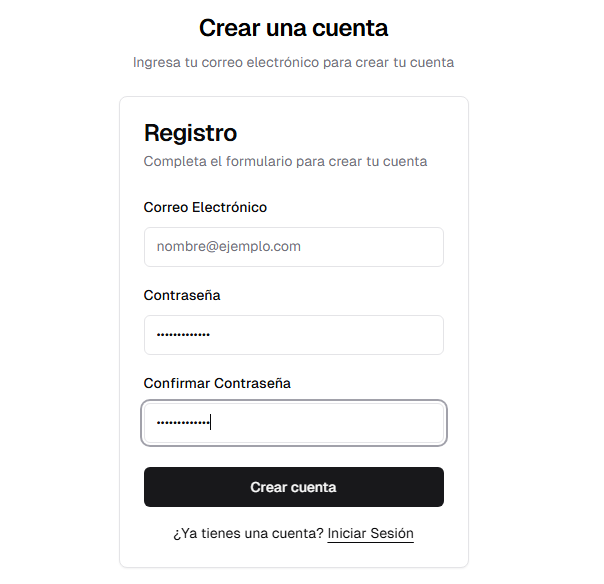
\includegraphics[width=0.6\textwidth]{images/create.PNG} % Imagen del ejemplo
			\end{center}
			\medskip % Espacio después de la imagen
		}
		
		
	\end{userstory}
	
	\begin{userstory}[hu:02]
		\storyname{Iniciar sesión en el sistema}
		\storyuser{Usuario registrado}
		\storyiter{1} % Iteración estimada
		\storypriority{Alta} % Basado en RF2
		\storyrisk{Bajo}
		\storypoints{1 semana} % Estimación basada en ejemplo
		\storyprogrammer{Daniel Rojas Grass}
		\storydescription{
			Como usuario registrado, debe poder iniciar sesión utilizando su correo electrónico y contraseña previamente registrados, mi historial de conversaciones y utilizar las capacidades completas del sistema de chat. (Corresponde principalmente a RF2, RF4)
			
			\textbf{Precondiciones:}
			\begin{itemize}
				\item El usuario tiene una cuenta previamente registrada en el sistema.
				\item El usuario no tiene una sesión activa.
				\item El usuario se encuentra en la página o sección de inicio de sesión del sitio web.
				\item El \textit{backend} está operativo y accesible.
			\end{itemize}
			
			\textbf{Flujo de acción:}
			\begin{enumerate}
				\item Usuario ingresa su dirección de correo electrónico y contraseña en el formulario del sitio web.
				\item Usuario envía el formulario.
				\item El sitio web envía las credenciales al \textit{endpoint} de autenticación del \textit{backend}.
				\item El \textit{backend} verifica las credenciales contra la base de datos.
				\item Si las credenciales son válidas, el \textit{backend} genera un token de sesión (e.g., JWT) y lo retorna al \textit{frontend}.
				\item Si las credenciales son inválidas, el backend retorna un error de autenticación.
				\item El \textit{frontend} almacena el token de sesión de forma segura (e.g., localStorage, sessionStorage o cookie HttpOnly).
				\item Si el inicio de sesión es exitoso, el \textit{frontend} redirige al usuario a la interfaz principal del chat. Si falla, muestra un mensaje de error ("Credenciales incorrectas").
			\end{enumerate}
		}
		\storyobservation{
			Utilizar HTTPS para la comunicación. Implementar medidas contra ataques de fuerza bruta (e.g., límites de intentos). El manejo del token en el \textit{frontend} debe seguir las mejores prácticas de seguridad.
		}
		\storyinterface{
			Formulario de inicio de sesión del sitio web:
			\par\medskip % Añade un pequeño espacio vertical
			\begin{center} % Para centrar la imagen
				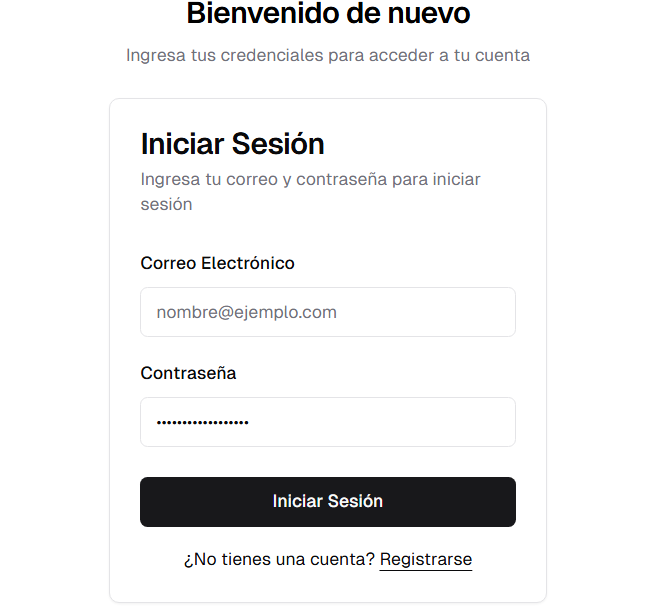
\includegraphics[width=0.6\textwidth]{images/loguin.PNG} % Imagen del ejemplo
			\end{center}
			\medskip
		}
		
	\end{userstory}
	
	\begin{userstory}[hu:03]
		\storyname{Cerrar sesión del sistema}
		\storyuser{Usuario autenticado}
		\storyiter{1} % Iteración estimada
		\storypriority{Media} % Basado en RF3
		\storyrisk{Bajo}
		\storypoints{0.5 semanas} % Estimación basada en ejemplo
		\storyprogrammer{Daniel Rojas Grass}
		\storydescription{
			Como usuario autenticado, debe disponer de una opción clara para cerrar su sesión activa, para asegurar la privacidad de su cuenta y finalizar su interacción con el sistema de forma segura. (Corresponde principalmente a RF3)
			
			\textbf{Precondiciones:}
			\begin{itemize}
				\item El usuario tiene una sesión activa (posee un token válido).
				\item El usuario está en la interfaz principal del sistema.
			\end{itemize}
			
			\textbf{Flujo de acción:}
			\begin{enumerate}
				\item Usuario hace clic en el botón o enlace 'Cerrar Sesión'.
				\item El \textit{frontend} elimina el token de sesión almacenado localmente.
				\item (Recomendado) El \textit{frontend} envía una solicitud al \textit{backend} para invalidar el token en el servidor (si se usa una blacklist de tokens).
				\item El \textit{frontend} redirige al usuario a la página de inicio de sesión o a una página pública principal.
				\item Cualquier intento posterior de acceder a rutas protegidas con el token antiguo debe fallar.
			\end{enumerate}
		}
		\storyobservation{
			El botón de cerrar sesión debe ser fácilmente accesible en la interfaz de usuario autenticado.
		}
		\storyinterface{Botón cerrar sesión en el sitio web:
			\par\medskip % Añade un pequeño espacio vertical
			\begin{center} % Para centrar la imagen
				
\includegraphics[width=0.6\textwidth]{images/cerrar.PNG} % Imagen del ejemplo
			\end{center}
		}
		
	\end{userstory}
	
	% ==========================================
	% Gestión de Conversaciones
	% ==========================================
	
	\begin{userstory}[hu:04]
		\storyname{Iniciar una nueva conversación}
		\storyuser{Usuario autenticado}
		\storyiter{2} % Iteración estimada
		\storypriority{Alta} % Basado en RF5
		\storyrisk{Bajo}
		\storypoints{0.5 semanas} % Estimación basada en ejemplo
		\storyprogrammer{Daniel Rojas Grass}
		\storydescription{
			Como usuario autenticado, debe poder iniciar una nueva conversación de chat en cualquier momento, para realizar consultas sobre temas distintos sin mezclar las interacciones o para empezar una nueva conversación si lo necesita. (Corresponde principalmente a RF5)
			
			\textbf{Precondiciones:}
			\begin{itemize}
				\item El usuario tiene una sesión activa.
				\item El usuario se encuentra en la interfaz principal del chat.
			\end{itemize}
			
			\textbf{Flujo de acción:}
			\begin{enumerate}
				\item Usuario hace clic en la opción "Nueva Conversación" (o icono '+').
				\item El \textit{frontend} limpia el área de visualización del chat actual.
				\item El \textit{frontend} establece un estado interno que indica que la próxima consulta pertenece a una nueva conversación (puede no requerir llamada inmediata al \textit{backend}).
				\item Opcionalmente, el \textit{frontend} puede asignar un ID temporal a la nueva conversación hasta que se envíe el primer mensaje.
				\item La interfaz se muestra lista para recibir la primera consulta de la nueva conversación.
			\end{enumerate}
		}
		\storyobservation{
			La acción debe ser visualmente clara y distinguible de seleccionar una conversación existente. El estado de "nueva conversación" debe manejarse correctamente hasta el primer envío.
		}
		\storyinterface{Botón nueva conversación en el sitio web:
			\par\medskip % Añade un pequeño espacio vertical
			\begin{center} % Para centrar la imagen
				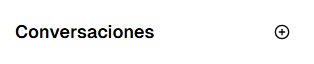
\includegraphics[width=0.6\textwidth]{images/newConversation.PNG} % Imagen del ejemplo
			\end{center}
			\medskip
		}
		
	\end{userstory}
	
	\begin{userstory}[hu:05]
		\storyname{Ver historial de conversaciones}
		\storyuser{Usuario autenticado}
		\storyiter{2} % Iteración estimada
		\storypriority{Media} % Basado en RF6
		\storyrisk{Bajo}
		\storypoints{1 semana} % Estimación basada en ejemplo
		\storyprogrammer{Daniel Rojas Grass}
		\storydescription{
			Como usuario autenticado, debe ver una lista organizada de sus conversaciones anteriores (por ejemplo, con un título autogenerado o fecha), para poder identificar y acceder fácilmente a interacciones pasadas. (Corresponde principalmente a RF6)
			
			\textbf{Precondiciones:}
			\begin{itemize}
				\item El usuario tiene una sesión activa.
				\item El \textit{backend} y la base de datos que almacena el historial están operativos.
			\end{itemize}
			
			\textbf{Flujo de acción:}
			\begin{enumerate}
				\item El \textit{frontend} (al cargar la interfaz principal o al interactuar con un panel de historial) solicita la lista de conversaciones del usuario al \textit{backend}.
				\item El backend consulta la base de datos para obtener los metadatos de las conversaciones asociadas al usuario autenticado (ID, título/fecha, última actualización).
				\item El \textit{backend} retorna la lista de conversaciones al \textit{frontend}.
				\item El \textit{frontend} muestra la lista en un panel lateral o sección designada, permitiendo al usuario ver los identificadores de cada conversación.
			\end{enumerate}
		}
		\storyobservation{
			Considerar paginación si el historial puede ser muy largo. La generación de títulos/identificadores debe ser útil (e.g., basado en la primera consulta). La lista debe actualizarse si se crea o elimina una conversación.
		}
		\storyinterface{Panel/Sección de Historial en el sitio web:
			\par\medskip % Añade un pequeño espacio vertical
			\begin{center} % Para centrar la imagen
				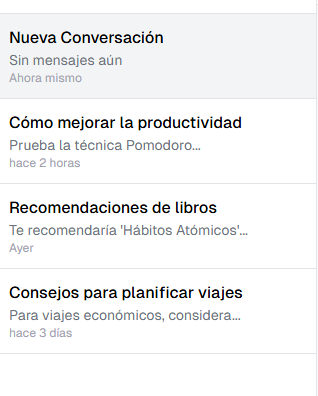
\includegraphics[width=0.4\textwidth]{images/histo.PNG} % Imagen del ejemplo
			\end{center}
			\medskip
		}
		
	\end{userstory}
	
	\begin{userstory}[hu:06]
		\storyname{Abrir una conversación del historial}
		\storyuser{Usuario autenticado}
		\storyiter{2} % Iteración estimada
		\storypriority{Media} % Basado en RF7
		\storyrisk{Bajo}
		\storypoints{1 semana} % Estimación basada en ejemplo
		\storyprogrammer{Daniel Rojas Grass}
		\storydescription{
			Como usuario autenticado, debe poder seleccionar una conversación específica de su historial listado, para cargar su contenido completo (consultas y respuestas) en la interfaz principal del chat y, opcionalmente, continuarla. (Corresponde principalmente a RF7)
			
			\textbf{Precondiciones:}
			\begin{itemize}
				\item El usuario tiene una sesión activa.
				\item El usuario está viendo la lista de su historial de conversaciones (HU:05).
				\item El \textit{backend} y la base de datos que almacena el historial están operativos.
			\end{itemize}
			
			\textbf{Flujo de acción:}
			\begin{enumerate}
				\item Usuario hace clic en una conversación específica en la lista del historial.
				\item El \textit{frontend} envía una solicitud al \textit{backend} pidiendo el contenido completo de la conversación seleccionada (pasando su ID).
				\item El \textit{backend} recupera todas las consultas y respuestas asociadas a esa conversación para ese usuario.
				\item El \textit{backend} retorna el historial completo de mensajes de esa conversación al \textit{frontend}.
				\item El \textit{backend} limpia el área de chat actual y muestra los mensajes recuperados en el orden correcto.
				\item El \textit{backend} establece la conversación seleccionada como la "conversación activa" actual.
				\item La interfaz permite al usuario añadir nuevas consultas a esta conversación activa.
			\end{enumerate}
		}
		\storyobservation{
			La carga debe ser eficiente, especialmente para conversaciones largas. La interfaz debe indicar claramente cuál conversación del historial está activa.
		}
		\storyinterface{Interacción con lista de historial y chat principal en el sitio web:
			\par\medskip % Añade un pequeño espacio vertical
			\begin{center} % Para centrar la imagen
				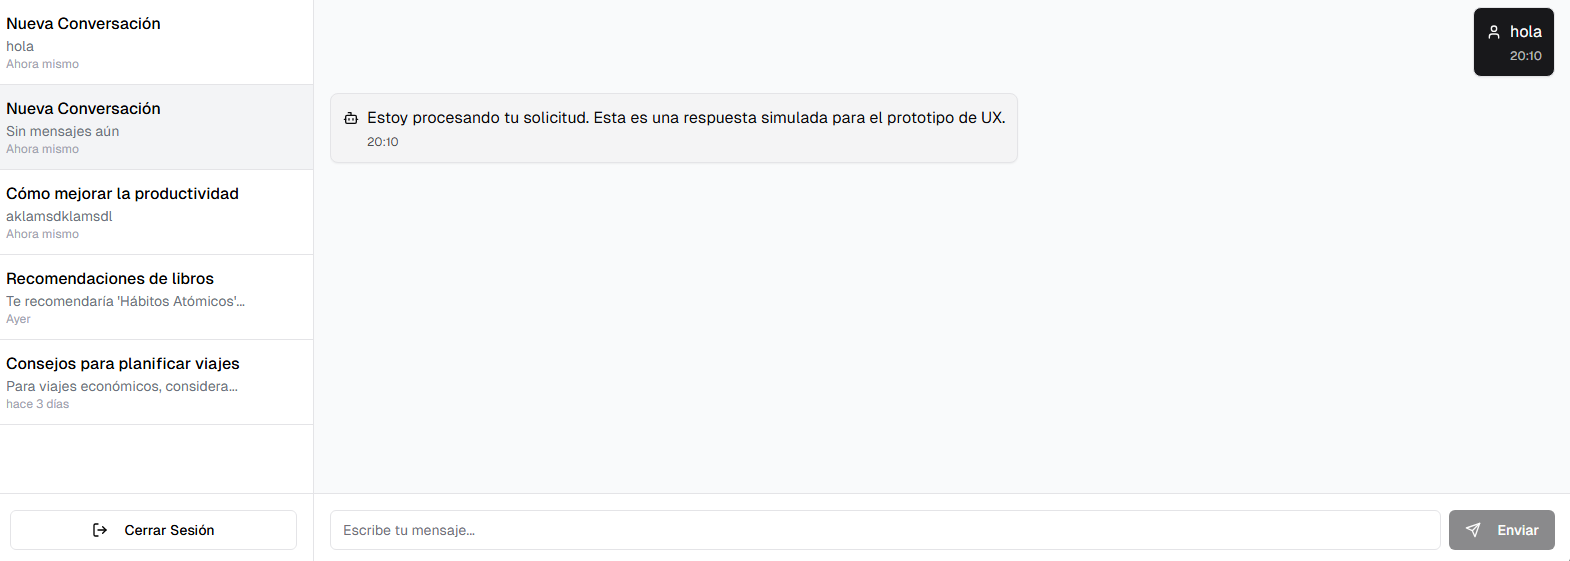
\includegraphics[width=0.6\textwidth]{images/lista.PNG} % Imagen del ejemplo
			\end{center}
			\medskip
		}
		
	\end{userstory}
	
	\begin{userstory}[hu:07]
		\storyname{Eliminar una conversación del historial}
		\storyuser{Usuario autenticado}
		\storyiter{3} % Iteración estimada
		\storypriority{Baja} % Basado en RF8
		\storyrisk{Bajo} % Riesgo de pérdida de datos si no hay confirmación
		\storypoints{1 semana} % Estimación basada en ejemplo
		\storyprogrammer{Daniel Rojas Grass}
		\storydescription{
			Como usuario autenticado, debe tener la opción de eliminar permanentemente una conversación específica de su historial, para mantener su historial limpio y relevante. (Corresponde principalmente a RF8)
			
			\textbf{Precondiciones:}
			\begin{itemize}
				\item El usuario tiene una sesión activa.
				\item El usuario está viendo la lista de su historial o tiene una conversación cargada que desea eliminar.
				\item El \textit{backend} y la base de datos que almacena el historial están operativos.
			\end{itemize}
			
			\textbf{Flujo de acción:}
			\begin{enumerate}
				\item Usuario hace clic en la opción "Eliminar" asociada a una conversación en la lista del historial (o en la conversación activa).
				\item El \textit{frontend} muestra un diálogo de confirmación ("¿Estás seguro de que quieres eliminar esta conversación? Esta acción no se puede deshacer.").
				\item Si el usuario confirma la eliminación:
				\begin{enumerate}
					\item El frontend envía una solicitud al backend DRF para eliminar la conversación (pasando su ID).
					\item El backend verifica que la conversación pertenece al usuario y la elimina de la base de datos.
					\item El backend retorna una respuesta de éxito al frontend.
					\item El frontend elimina la conversación de la lista visible en el historial.
					\item Si la conversación eliminada era la activa, el frontend limpia el área de chat o carga una conversación por defecto/nueva.
				\end{enumerate}
				\item Si el usuario cancela, no se realiza ninguna acción.
			\end{enumerate}
		}
		\storyobservation{
			La confirmación es crucial para prevenir eliminaciones accidentales. La eliminación debe ser lógicamente completa en el backend (borrado permanente).
		}
		\storyinterface{Opción de Eliminar en la lista de Historial o Chat activo:
			\par\medskip % Añade un pequeño espacio vertical
			\begin{center} % Para centrar la imagen
				
\includegraphics[width=0.6\textwidth]{images/eliminarC.PNG} % Imagen del ejemplo (asumiendo que muestra un icono/botón de eliminar)
			\end{center}
			\medskip
		}
		
	\end{userstory}
	
	
	\chapter{Targetas CRC}
		
		\begin{longtable}{|l|l|}
			\caption{Tarjeta CRC: Usuario} \label{tablacrc6} \\
			\hline
			\multicolumn{2}{|c|}{\textbf{Tarjeta CRC}} \\
			\hline
			\textbf{Clase} & \textbf{Usuario} \\
			\hline
			\parbox[t]{0.45\linewidth}{\textbf{Responsabilidades:} \\ 
				Proporcionar datos para registro (email, username, contraseña) \\ 
				Almacenar credenciales de forma segura \\ 
				Mantener información de sesión activa \\ 
				Asociar conversaciones al usuario} 
			& 
			\parbox[t]{0.45\linewidth}{\textbf{Colaboración:} \\ 
				Autenticador \\ 
				BaseDeDatos \\ 
				Conversación} \\
			\hline
		\end{longtable}
		
		\begin{longtable}{|l|l|}
			\caption{Tarjeta CRC: Autenticador} \label{tablacrc7} \\
			\hline
			\multicolumn{2}{|c|}{\textbf{Tarjeta CRC}} \\
			\hline
			\textbf{Clase} & \textbf{Autenticador} \\
			\hline
			\parbox[t]{0.45\linewidth}{\textbf{Responsabilidades:} \\ 
				Validar datos de registro (email único, contraseña fuerte) \\ 
				Autenticar credenciales de inicio de sesión \\ 
				Generar y gestionar tokens de sesión \\ 
				Finalizar sesiones activas} 
			& 
			\parbox[t]{0.45\linewidth}{\textbf{Colaboración:} \\ 
				Usuario \\ 
				BaseDeDatos \\ 
				Backend} \\
			\hline
		\end{longtable}
		
		\begin{longtable}{|l|l|}
			\caption{Tarjeta CRC: Conversación} \label{tablacrc8} \\
			\hline
			\multicolumn{2}{|c|}{\textbf{Tarjeta CRC}} \\
			\hline
			\textbf{Clase} & \textbf{Conversación} \\
			\hline
			\parbox[t]{0.45\linewidth}{\textbf{Responsabilidades:} \\ 
				Iniciar una nueva sesión de chat \\ 
				Almacenar consultas y respuestas \\ 
				Permitir continuación de una conversación existente \\ 
				Eliminar una conversación del historial} 
			& 
			\parbox[t]{0.45\linewidth}{\textbf{Colaboración:} \\ 
				Usuario \\ 
				Historial \\ 
				Backend \\ 
				BaseDeDatos} \\
			\hline
		\end{longtable}
		
		\begin{longtable}{|l|l|}
			\caption{Tarjeta CRC: Historial} \label{tablacrc9} \\
			\hline
			\multicolumn{2}{|c|}{\textbf{Tarjeta CRC}} \\
			\hline
			\textbf{Clase} & \textbf{Historial} \\
			\hline
			\parbox[t]{0.45\linewidth}{\textbf{Responsabilidades:} \\ 
				Listar todas las conversaciones de un usuario \\ 
				Proporcionar metadatos de conversaciones (título, fecha) \\ 
				Permitir selección de una conversación específica} 
			& 
			\parbox[t]{0.45\linewidth}{\textbf{Colaboración:} \\ 
				Usuario \\ 
				Conversación \\ 
				Backend \\ 
				BaseDeDatos} \\
			\hline
		\end{longtable}
		
		\begin{longtable}{|l|l|}
			\caption{Tarjeta CRC: Chat} \label{tablacrc10} \\
			\hline
			\multicolumn{2}{|c|}{\textbf{Tarjeta CRC}} \\
			\hline
			\textbf{Clase} & \textbf{Chat} \\
			\hline
			\parbox[t]{0.45\linewidth}{\textbf{Responsabilidades:} \\ 
				Mostrar la interfaz de chat activo \\ 
				Permitir ingreso de consultas en lenguaje natural \\ 
				Visualizar consultas y respuestas (texto e imágenes) \\ 
				Indicar estado de procesamiento} 
			& 
			\parbox[t]{0.45\linewidth}{\textbf{Colaboración:} \\ 
				Conversación \\ 
				Backend \\ 
				MicroservicioMAS} \\
			\hline
		\end{longtable}
		
		\begin{longtable}{|l|l|}
			\caption{Tarjeta CRC: Backend} \label{tablacrc11} \\
			\hline
			\multicolumn{2}{|c|}{\textbf{Tarjeta CRC}} \\
			\hline
			\textbf{Clase} & \textbf{Backend} \\
			\hline
			\parbox[t]{0.45\linewidth}{\textbf{Responsabilidades:} \\ 
				Gestionar endpoints REST para autenticación y chat \\ 
				Coordinar comunicación entre frontend y MicroservicioMAS \\ 
				Almacenar y recuperar datos de conversaciones \\ 
				Proteger rutas con autenticación} 
			& 
			\parbox[t]{0.45\linewidth}{\textbf{Colaboración:} \\ 
				Usuario \\ 
				Autenticador \\ 
				Conversación \\ 
				Historial \\ 
				Chat \\ 
				MicroservicioMAS \\ 
				BaseDeDatos} \\
			\hline
		\end{longtable}
		
		\begin{longtable}{|l|l|}
			\caption{Tarjeta CRC: BaseDeDatos} \label{tablacrc12} \\
			\hline
			\multicolumn{2}{|c|}{\textbf{Tarjeta CRC}} \\
			\hline
			\textbf{Clase} & \textbf{BaseDeDatos} \\
			\hline
			\parbox[t]{0.45\linewidth}{\textbf{Responsabilidades:} \\ 
				Almacenar datos de usuarios (credenciales, sesiones) \\ 
				Persistir conversaciones y su historial \\ 
				Proveer acceso a datos del \textit{Diario de la Marina} (vectorial y CSV)} 
			& 
			\parbox[t]{0.45\linewidth}{\textbf{Colaboración:} \\ 
				Usuario \\ 
				Autenticador \\ 
				Conversación \\ 
				Historial \\ 
				Backend \\ 
				Agente Recuperador (FAISS) \\ 
				Agente PandasAi} \\
			\hline
		\end{longtable}
		
		\begin{longtable}{|l|l|}
			\caption{Tarjeta CRC: MicroservicioMAS} \label{tablacrc13} \\
			\hline
			\multicolumn{2}{|c|}{\textbf{Tarjeta CRC}} \\
			\hline
			\textbf{Clase} & \textbf{MicroservicioMAS} \\
			\hline
			\parbox[t]{0.45\linewidth}{\textbf{Responsabilidades:} \\ 
				Recibir consultas del backend \\ 
				Coordinar agentes internos para procesar consultas \\ 
				Devolver respuestas procesadas (texto e imágenes) al backend} 
			& 
			\parbox[t]{0.45\linewidth}{\textbf{Colaboración:} \\ 
				Backend \\ 
				Agente Moderador \\ 
				Agente Recuperador (FAISS) \\ 
				Agente Contextualizador \\ 
				Agente de Validación \\ 
				Agente PandasAi} \\
			\hline
		\end{longtable}
		
		
		
		
\end{addendum}
 % Anexos
	
	% Bibliografía
	\renewcommand\bibname{Referencias bibliográficas}
	\bibliographystyle{IEEEtran}
	\bibliography{library}\label{bibliography}
	
\end{document}
